%!TEX root =  ../final-report.tex

% Chapters are setup to start on a new page.
% The short version of that title appears in square brackets. This is used for the table of contents listing. 
% The long version of the title has a command "\setstretch{0.5}" in order to reduce the line spacing in the
% title and then the title text.
\section{DC Switching and Power Integration}

DC circuits are commonly used for controlling RF switches due to the cheaper cost in comparison to their RF counterparts and the reduction in frequency interference due to the maximum attenuation of any frequency components at DC. For our design we need a DC circuit for address decoding of the RF switch. In effect, the function of the DC switch is to set the control parameters in order to specify what the response of the RF switch will be at that point in time. 

\subsection{Research and Design}

\subsubsection{DC Switch}

At the onset of the project, we examined the previous switch design to understand how it would integrate with the RF switch and set the control parameters for the acquisition of data by the VNA. Our goal was to improve upon this design so that it was feasible with the new system we wanted to implement.

\subsubsection{Hardware}

The initial design appeared very complex and cumbersome to deduce because it had wires everywhere. The first task was therefore to ascertain the possibility of having a neater hardware with very minimal adjustment to the circuit after the printing of the PCB. This meant that most of the design should be implemented in the PCB in order to reduce complexity and make troubleshooting easier. This also ensure a reduction in noise cause by all the numerous wiring and addition electrical components that was everywhere.

Figure \ref{fig:eddie_fig1} highlights that function of the DC switch in perfect simplicity. The control parameters are letters from A – L and these are sourced from the DC switch to the SP3Ts, SP3Ts and SPDTs of the RF switch

\begin{figure}[h]
	\begin{center}
		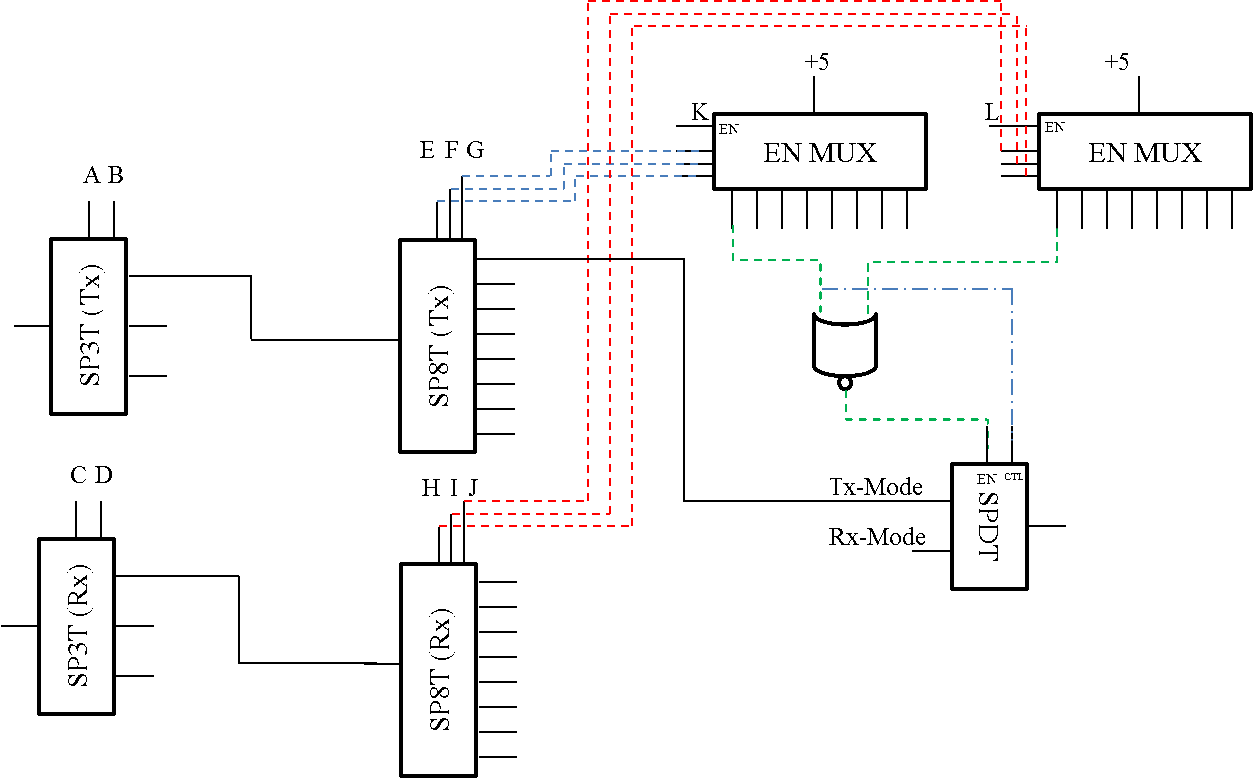
\includegraphics[width=4.5in]{./images/eddie_image1.png}
		\caption{}
		\label{fig:eddie_fig1}
	\end{center}
\end{figure}


\subsubsection{Software}

The software control of the DC switching circuit is done by an Arduino microcontroller loaded with a table that references the control lines for each multiplexer. This allows the SPDTs to function as an input or an output depending on the values set on the control lines but the Arduino. And will be concurrent with the presents action of the VNA such that, only one SPDT is in transmit mode at a given time. The software will also turn on one the SP8T for transmission of the signal and turn the other SP8Ts responsible for reception of the signals. 

After the research and understanding of requirements were satisfied, a truth table was drawn in order to simplify the circuit to its least possible scenario where the fewest components are used to achieve the expected results. This truth table was then transcribed into code for and then loaded unto the Arduino. This Arduino was set to function in synchronism with the raspberry pie.

\subsubsection{ESD Protection}

Any reliable system design requires some form of Electrostatic Discharge protection. Choosing the right circuit protection device involves considering criteria such as: Response time, ESD current handling capacity and, maximum reverse leakage current. Also the device should not interfere with the normal operation of the circuit. Designing the DC circuit also meant taking the RF circuit into consideration in order to minimize electrostatic discharge and current leakage. 

We considered N-well resisters, gate-grounded and gate-coupled protection options, silicon controlled rectifiers and diodes. Ultimately we decided to use diodes and capacitors due to its simplicity.

\subsubsection{Power Integration}

A portable power source will be integrated into our data collection unit to provide enough electrical power to run the VNA and the switch box simultaneously for the duration of time it takes to gather the parametric information from the VNA. 12V rechargeable battery which produces 3.0Ah of current will be hour choice as our power source.

\subsection{Design and Implementation}

\subsubsection{DC Switch}

The design of the switch required the use of Altium and the Arduino user interface. The hardware was designed in Altium and the software was writing in the Arduino mainframe in the C++ programing language 

\subsubsection{Hardware}

Designing the PCB first started with the schematic and a review of the schematic to ensure its accuracy. Figre \ref{fig_eddie_fig2} shows the final schematic that was used in the printing of the PCB in Altium.

\begin{figure}[h]
	\begin{center}
		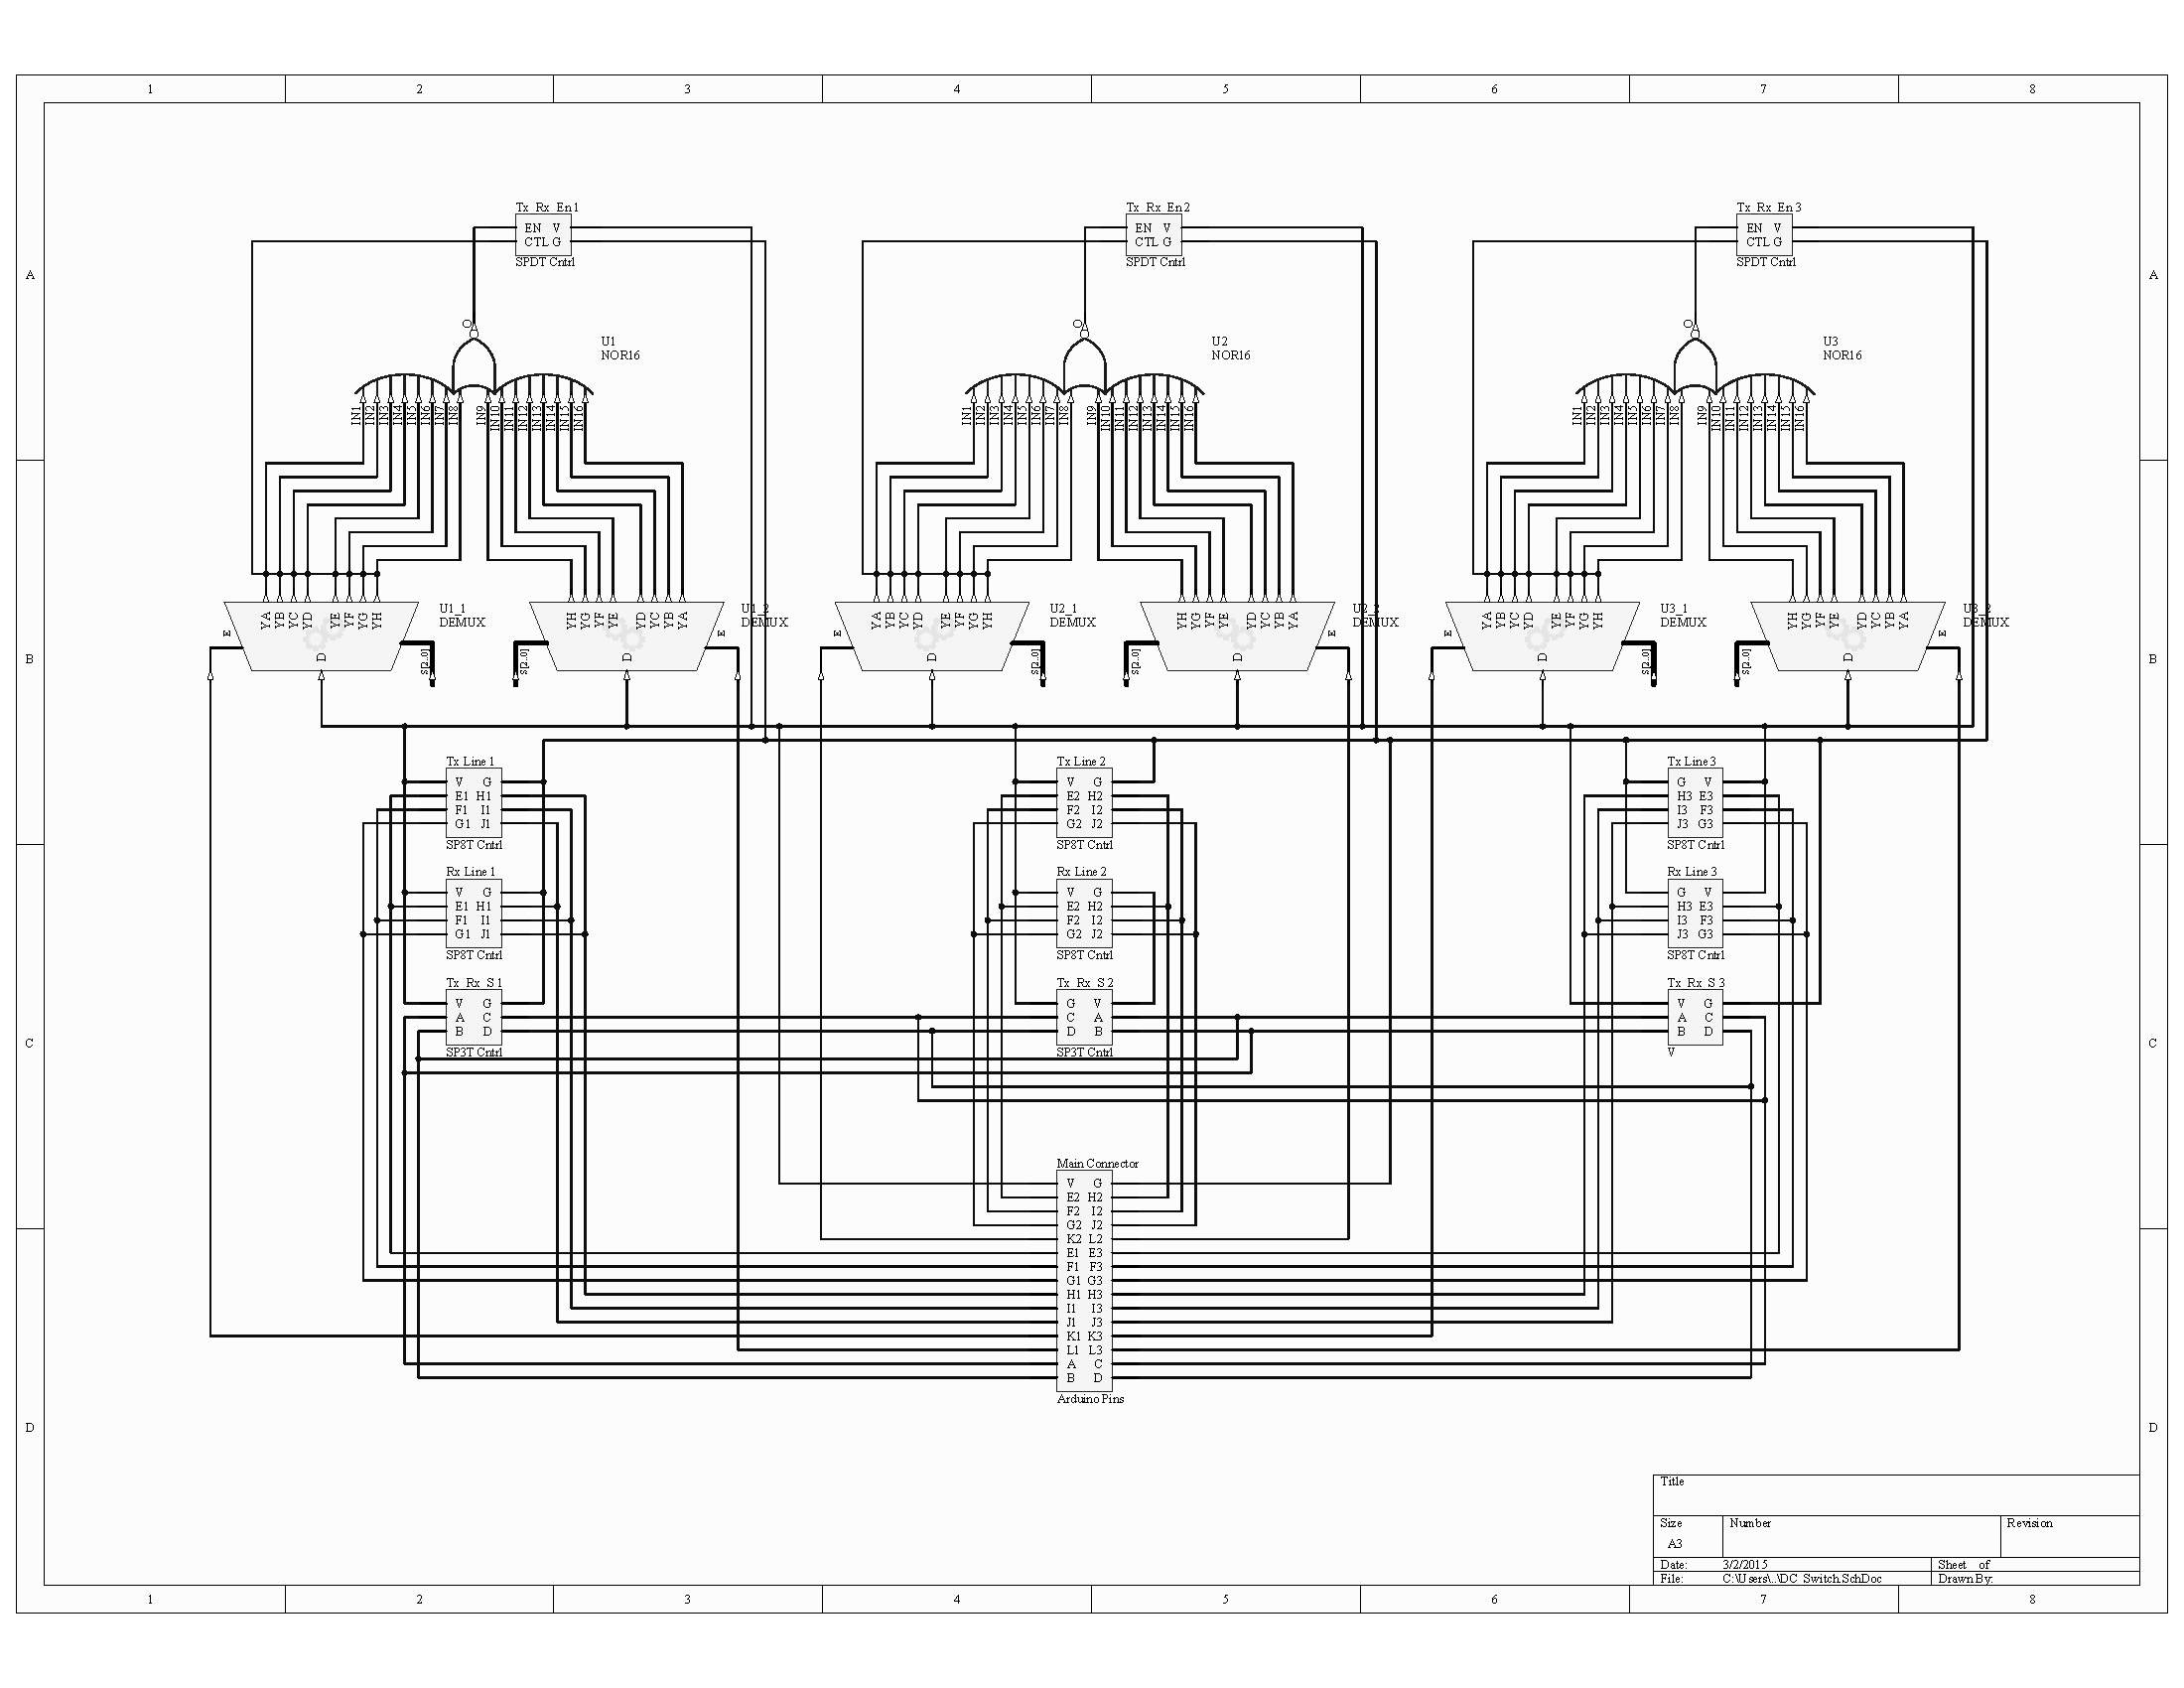
\includegraphics[width=5.5in]{./images/eddie_image2.png}
		\caption{}
		\label{fig:eddie_fig2}
	\end{center}
\end{figure}









